\documentclass[12pt,a4paper,fleqn]{article}
\usepackage[utf8]{inputenc}
\usepackage[russian]{babel}
\usepackage{amssymb, amsmath, multicol}
\usepackage{enumitem}
\usepackage{lipsum}
\usepackage{euler}
\oddsidemargin=-15.4mm
\textwidth=190mm
\headheight=-32.4mm
\textheight=277mm
\parindent=0pt
\parskip=8pt
\pagestyle{empty}
\usepackage{graphicx}
\begin{document}
\begin{center}
\textbf{\LARGE{Исследовательская работа по теме:\\Исследование функции дифференциальными методами}}\end{center}\newpage\textbf{\LARGE Глава I. Функция}

\begin{center}
$y = $$x^{cos(x)}$

\end{center}
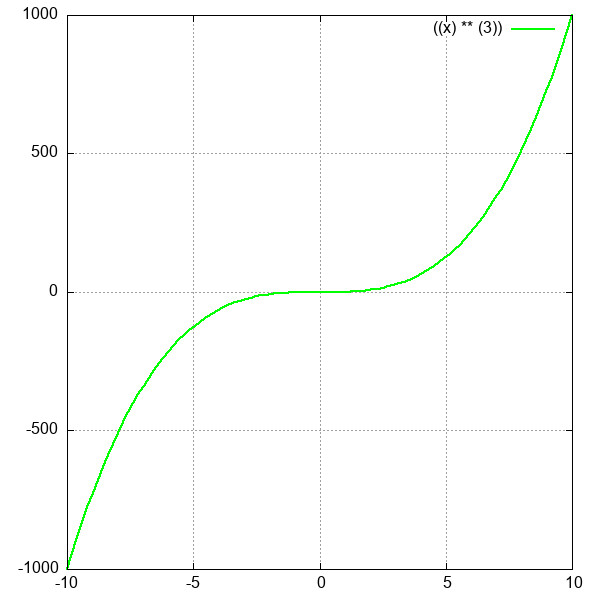
\includegraphics{GraphicDumps/plot.jpg}\newpage \textbf{\LARGE Глава II. Визуальный анализ функции}

От коробки до нк все знают, что

\begin{center}
$y = $$x^{cos(x)}$

\end{center}
\newpage \textbf{\LAGRE Глава III. Дифференцирование}

Segmentation fault (core dumped)

\begin{center}
 ($x)'
  = 1$\end{center}
Если посмотреть на выражение под другим углом, можно получить

\begin{center}
 ($x)'
  = 1$\end{center}
Говорят

\begin{center}
 ($cos(x))'
  = (1 \cdot (0 - sin(x)))$\end{center}
С другой стороны

\begin{center}
A = $((\frac{cos(x)}{x} \cdot 1) + ((1 \cdot (0 - sin(x))) \cdot log(x)))$\end{center}
\begin{center}
 ($x^{cos(x)})'
  = (x^{cos(x)} \cdot A)$\end{center}
\newpage \textbf{\LARGE Глава IV.Упрощение выражения}

Таким образом

\begin{center}
$(\frac{cos(x)}{x} \cdot 1) = \frac{cos(x)}{x}$\end{center}
Руководствуясь базовой логикой, получаем

\begin{center}
$(1 \cdot (0 - sin(x))) = (0 - sin(x))$\end{center}
\newpage \textbf{\LARGE Глава V. Полученая производная}

$y = $$x^{cos(x)}$

\begin{center}
A = $(\frac{cos(x)}{x} + ((0 - sin(x)) \cdot log(x)))$\end{center}
$y' = $$(x^{cos(x)} \cdot A)$

\includegraphics{GraphicDumps/plot_1.jpg}
\end{document}